\chapter{Marco Teórico}
\newpage
\section{Panorama Internacional de las fuentes de energia renovables}
La importancia del impulso a las energías renovables y la eficiencia energética no sólo estriba en reducir la dependencia en la utilización de los combustibles fósiles; también se han creado nuevas oportunidades económicas y se ha desarrollado un mercado energético totalmente diversificado y más amigable con el medio ambiente.\\

Durante la década pasada, y particularmente en años recientes, han sido posibles avances en tecnologías de energía renovable, incrementos en la capacidad de generación a nivel mundial, así como rápidas reducciones de costos gracias al apoyo brindado por las políticas económicas, mismas que han atraído una cantidad significativa de inversiones e impulsado la baja de costos, por medio de economías de escala.\\

2015 fue un año trascendental para el desarrollo de las energías renovables a nivel mundial, en muchos países se ha dado un sustancial incremento de la capacidad instalada con fuentes renovables, derivado del aumento de la rentabilidad de las tecnologías renovables.\\

Hoy en día, gracias a las políticas aplicadas en las economías en desarrollo, se ha da acceso a financiamientos que permitan la incorporación de un sistema energético totalmente modernizado, eficiente y respetuoso con el medio ambiente. Durante la 21ª. Conferencia de las Partes (COP 21) en París, Convención Marco de las Naciones Unidas sobre el cambio climático (UNFCCC por sus siglas en inglés), 195 países acordaron limitar el calentamiento global por debajo de los dos grados centígrados. Para ello, se requiere instrumentos precisos como: acelerar del uso de las energías renovables e incrementar los mecanismos de eficiencia energética.\\

Según cifras de International Renewable Energy Agency (IRENA, por sus siglas en ingles), a nivel mundial la capacidad instalada con energías renovables en 2015 fue de 503.8 GW. Las regiones con mayor participación de energías renovables son Asia con el 39.7\% y Europa con 25.1\% del total mundial, mientras que la región con menor participación es Centroamérica y el Caribe con 0.6\%. Por tipo de tecnología, la energía hidráulica concentro el 61.5\% del total de capacidad mundial, seguido de la energía eólica con 21.2\%, energía solar con 11.4\%, 5.2\% bioenergía y el restante 0.7\% se atribuye a tecnologías con energía geotérmica y marina.\\

En América Latina y el Caribe, gracias a la diversidad energética con la que cuenta, existe uno de los mercados de energía renovables más dinámicos del mundo. Al cierre del 2015, la capacidad de generación por energías renovables fue 212.4 GW de la cual, la energía hidráulica representó la mayor participación del total regional con una capacidad instalada de 172 GW proveniente de grandes plantas mayores a 10 MW.\\

La generación de energía eléctrica con energías renovables en esta región en 2014 fue de 817 TWh, siendo la energía hidroeléctrica la que concentró la mayor parte con 720 TWh, seguido de la bioenergía con 61 TWh y otras industrias de procesamiento forestal. La energía eólica representó 25 TWh de generación de electricidad, seguida de energía geotérmica y solar con 10 TWh y 1.5 TWh respectivamente. Entre el año 2000 al 2014, la diversidad de energías renovables utilizadas para generar electricidad han aumentado significativamente, como se muestra en la siguiente figura \ref{2000}. 

\begin{figure}[!h]
	\centering
	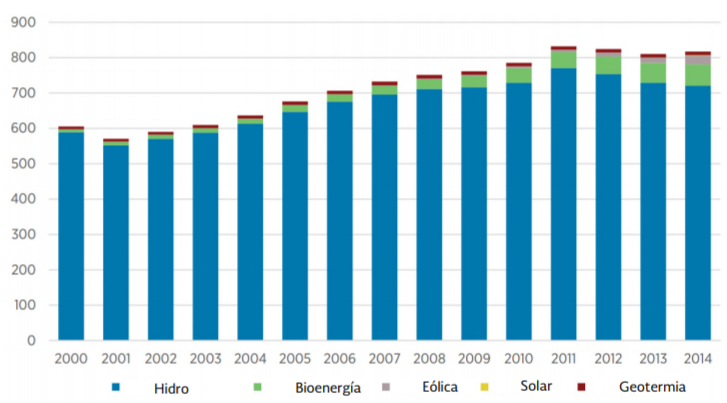
\includegraphics[width=10cm]{img/produccion.png}
	\caption{Evolución de la generación de electricidad en LatinoAmérica, 2000-2014. Fuente: Renewables in Latin American and the Caribbean, IRENA}
	\label{2000}
\end{figure}

\subsection{Las Energías Renovables en la Matriz Energética.}

La reducción en los costos, especialmente para la energía solar y eólica han permitido un considerable incremento en la participación de las energías renovables como fuentes de generación de energía limpia, aunado a esto, las políticas de apoyo para las energías renovables en México, derivadas de la Reforma Energética, han contribuido al fortalecimiento del mercado energético haciendo que las energías renovables sean altamente competitivas con los combustibles convencionales en el sector eléctrico.

\subsection{Potencial de Energías Renovables.}
El poder identificar zonas con alto potencial de energías renovables permite a los desarrolladores e interesados, invertir en proyectos que conlleven a la diversificación de la matriz energética.\\

De acuerdo al Inventario Nacional de Energías Renovables (INERE), el mayor potencial probado para generación de electricidad, es decir, aquel que cuenta con estudios técnicos y económicos que comprueban la factibilidad de su aprovechamiento, se encuentra en las energías eólica y solar.\\

El mayor potencial probable identificado, aquel que cuenta con estudios de campo que comprueban la presencia de los recursos, pero que no son suficientes para evaluar la factibilidad técnica y económica de explotación, corresponde a los recursos geotérmicos.\\

El mayor potencial posible se refiere al potencial teórico de los recursos pero que carece de los estudios necesarios para evaluar la factibilidad técnica y los posibles impactos económicos, ambientales y sociales. En este rubro el mayor potencial está en la energía solar seguida de la eólica.

\subsection{Avances en Energías Renovables}
Al cierre de 2015 la capacidad instalada de generación mediante energías renovables se incrementó 6.6\% respecto al periodo 2014, llegando a los 17,140.4 MW, lo cual representó el 25.2\% de la capacidad de generación total. La mayor parte de la capacidad en operación renovable continúa dominada por la generación hidroeléctrica, que en suma con la energía eólica representan el 80\% de la capacidad instalada en energías limpias. Entre 2005 y 2015, la energía eólica ha presentado la mayor expansión en capacidad instalada con el 104.7\% anual. Sin embargo, la energía hidráulica presenta la mayor concentración en la participación total de capacidad instalada con fuentes renovables, pero ha mantenido un ritmo de crecimiento de 1.7\% anual, como se muestra en la figura \ref{instalacion} a continuación.

\begin{figure}[!h]
	\centering
	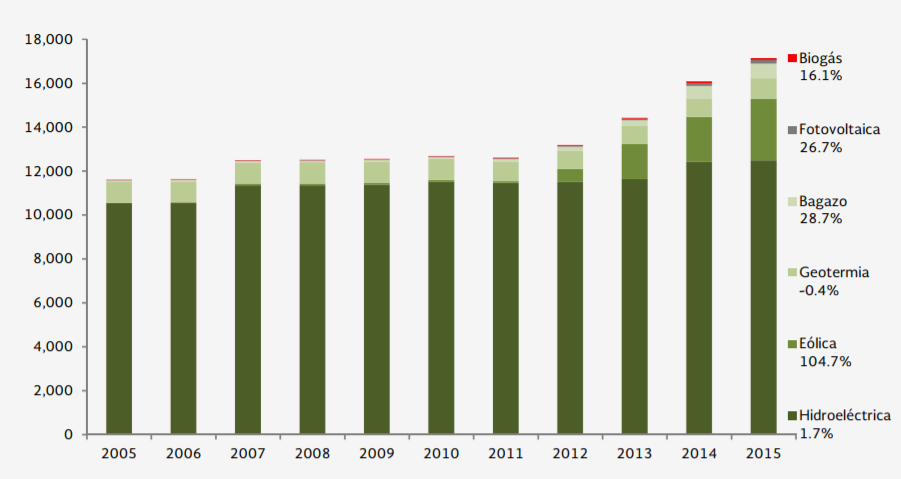
\includegraphics[width=10cm]{img/instalacion.png}
	\caption{Evlución de la capacidad instalada con enrgías renovables, 2005-2015.Fuente: SENER}
	\label{instalacion}
\end{figure}

\subsection{Generación Eléctrica con Energía Eólica.}
En los últimos cuatro años, la generación de energía eólica ha mostrado un crecimiento anual promedio equivalente a 2,330 GWh. Al cierre del 2015 la capacidad instalada alcanzó los 2,805.1 MW, lo que significó un incremento del 37.75\% respecto del 2014. En 2015, la generación eólica fue de 8,745.1 GWh, 36.08\% mayor a la generada en 2014. La generación de energía eléctrica a través de la energía eólica ha crecido significativamente desde 2005, de 5.0 GWh/año a 8,745.1 GWh, lo que representa un incremento de cerca del 174,802.0\%, clasificándose así en la segunda fuente de generación renovable (véase figura \ref{eolica}).

\begin{figure}[!h]
	\centering
	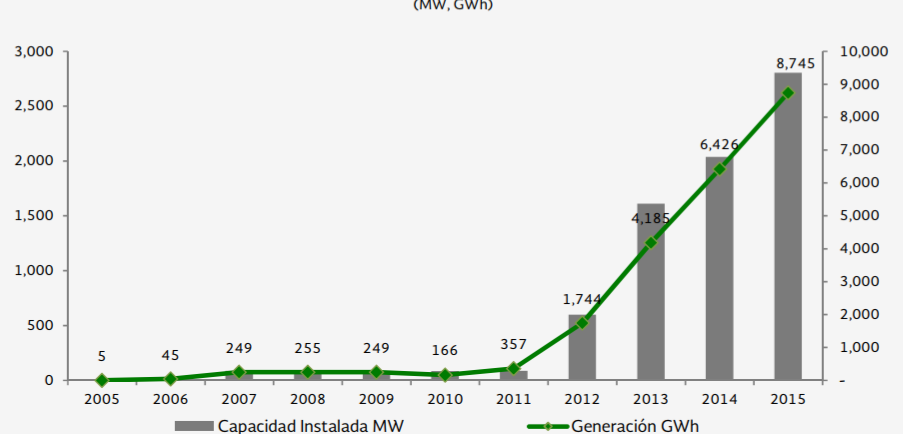
\includegraphics[width=10cm]{img/eolica.png}
	\caption{Capacidad instalada y generaciòn bruta de centrales eólica, 2005-2015. Fuente SENER}
	\label{eolica}
\end{figure}

\subsection{Generación Eléctrica con Energía Solar Fotovoltaica.}
Desde la publicación del Primer Contrato de Interconexión para Fuente de Energía Solar en Pequeña Escala, así como la entrada en operación de la primera central fotovoltaica de gran escala en 2011, la capacidad instalada y la generación de energía eléctrica a partir de energía solar se incrementó de 18.5 MW y 8.8 GWh en el año 2007 a 170.24 MW y 190.26 GWh en el año 2015. Este incremento se ha visto reforzado por el crecimiento importante de los Contratos de Interconexión Legados (Pequeña y Mediana Escala), los cuales desde 2010 han observado tasas de crecimiento importantes. (véase figura \ref{solar}).

\begin{figure}[!h]
	\centering
	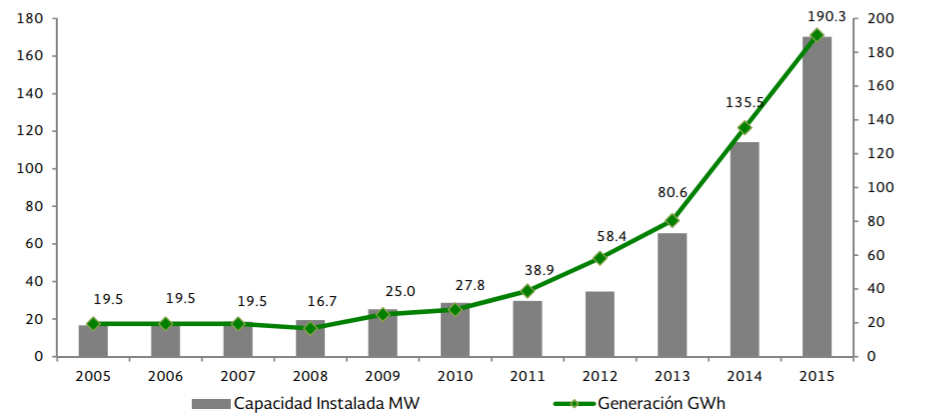
\includegraphics[width=10cm]{img/solar.png}
	\caption{Capacidades instaladas y generación bruta de centrales solares fotovoltaicas, 2005- 2015. Fuente: SENER}
	\label{solar}
\end{figure}

\section{Power TAC(Trading Agent Competition).}

Power TAC es una competencia de simulación de futuros mercados minoristas de energía eléctrica, en los que los competidores broker o agentes minoristas que compran y venden energía tanto en los mercados mayoristas como minoristas. El mercado al por mayor es una abstracción de los típicos mercados diurnos en Norteamérica y Europa, y el mercado al por menor es un mercado de tarifas, en el que los clientes pueden elegir entre ofertas de contratos de tarifas ofrecidos por los agentes. Los clientes son modelos de usuarios domésticos, empresariales e institucionales de energía eléctrica, así como pequeños productores de energía que poseen paneles solares o turbinas eólicas.\\

La primera competencia de Power TAC se celebro en año 2012 como parte de ka decimotercera competencia anual de agentes de comercio, durante al conferencia de AAMAS-12\footnote{The International Conference on Autonomous Agents and Multi-Agent Systems es la conferencia científica líder para la investigación en las áreas de inteligencia artificial, agentes autónomos y sistemas multiagentes.}. Los participantes diseñaron agentes  que actuaban como minoristas, obteniendo ganancia mediante la creación contratos y el comercio en le mercado al por mayor. La primera competencia de Power TAC se celebro en año 2012 como parte de ka decimotercera competencia anual de agentes de comercio, durante al conferencia de AAMAS-12. Los participantes diseñaron agentes  que actuaban como minoristas, obteniendo ganancia mediante la creación contratos y el comercio en le mercado al por mayor. El entorno  de simulación proporcionaba una gama de problemas para los agentes, incluyendo un mercado de energía al por mayor para el día a día, pronósticos de tiempo realistas que afectan la producción de energía eólica y solar, así como el consumo una variedad de preferencias sobre términos de tarifas y una distribuidor de utilidades que cobra por el transporte de energía y por desequilibrios entre la oferta y la demanda.\\

Una segunda ronda de Power TAC 2012 se celebró del 24 al 27 de septiembre de 2012, y la tercera ronda se celebró del 30 de noviembre al 7 de diciembre. Posteriormente las competencias se fueron realizando cada año con diferentes participantes (véase la tabla \ref{tab:competition}).

\begin{table}[!h]
	\begin{center}
		\begin{tabular}{|p{1cm}|p{7cm}|p{4cm}|}\hline
			\textbf{Año} & \textbf{Participantes} & \textbf{Ranking} \\ \hline
			2013
			&
			\begin{tabular}{p{7cm}}
			Aston University\\
			University of Zagreb\\
			INAOE\\
			University of Freiburg\\
			Aristotle University of Thessalonik\\
			UT Austin\\
			CWI Amsterdam\\
		\end{tabular}
		&
		\begin{tabular}{p{4cm}}
			1 TacTex         \\
			2 cwiBroker      \\
			3 MLLBroker      \\
			4 CrocodileAgent \\
			5 AstonTAC       \\
			6 Mertacor       \\
			7 INAOEBroker02  \\
		\end{tabular}
		\\ \hline
																						
		2014
		&
		\begin{tabular}{p{7cm}}
			Universitaet Duisburg-Essen          \\
			University of Zagreb                 \\
			Westfaelische Hochschule             \\
			Aristotle University of Thessaloniki \\
			UT Austin                            \\
			INAOE                                \\
			CWI Amsterdam                        \\
		\end{tabular}
		&
		\begin{tabular}{p{4cm}}
			1 AgentUDE       \\
			2 cwiBroker      \\
			3 CrocodileAgent \\
			4 Maxon          \\
			5 Mertacor       \\
			6 coldbroker     \\
		\end{tabular}
		\\ \hline
																		
		2015
		&
		\begin{tabular}{p{7cm}}
			Universitaet Duisburg-Essen          \\
			INAOE                                \\
			The Chinese University of Hong Kong  \\
			University of Zagreb                 \\
			Westfaelische Hochschule             \\
			Aristotle University of Thessaloniki \\
			Nanyang Technological University     \\
			UTEP/NMSU                            \\
			Hebrew University of Jerusalem       \\
			UT Austin                            \\
			CWI Amsterdam                        \\
		\end{tabular}
		&
		\begin{tabular}{p{4cm}}
			1 Maxon15         \\
			2 TacTex          \\
			3 CUHKTac         \\
			4 AgentUDE        \\
			5 Sharpy          \\
			6 COLDPower       \\
			7 cwiBroker       \\
			8 Mertacor        \\
			9 NTUTacAgent     \\
			10 SPOT           \\
			11 CrocodileAgent \\
		\end{tabular}
		\\ \hline
																	
		2016
		&   
		\begin{tabular}{p{7cm}}
			The Chinese University of Hong Kong  \\  
			Universitaet Duisburg-Essen          \\
			INAOE                                \\
			University of Zagreb                 \\
			Aristotle University of Thessaloniki \\
			UTEP/NMSU                            \\
			Westfaelische Hochschule             \\
		\end{tabular}
		&
		\begin{tabular}{p{4cm}}
			1 maxon16        \\
			2 COLDPower      \\
			3 AgentUDE       \\
			4 SPOT           \\
			5 Mertacor       \\
			6 AgentCU        \\
			7 CrocodileAgent \\
		\end{tabular}
		\\ \hline
																								
		\end{tabular}			
	\end{center}
	\caption{Competencias realizadas por Power TAC 2013-2017.}
	\label{tab:competition}
\end{table}

El entorno de simulación de Power TAC modela un mercado  minorista y mayorista, una entidad de distribución y regularización y una población de clientes de producción y de consumo, situado en una ubicación real en la Tierra durante un periodo especifico con datos meteorológico reales. El mercado al por mayor es un mercado de llamadas relativamente simple, similar a muchos de los mercados ya existentes de energía eléctrica. Los modelos clientes incluyen hogares, vehículos electrónicos y entidades comerciales e industriales, ademas algunos de los clientes tienen capacidades de producción a partir de paneles solares y de turbinas eólicas. El distribuidor de utilidades modela un monopolio de regularización que posee  una red de distribución local y es responsable del mantenimiento de la infraestructura. El balance entre la oferta y la demandad en tiempo real es gestionado por u mecanismo basado en un mecanismo de incentivos económicos para alentar a los broker a mantener un equilibrio dentro de su portafolio de clientes de producción y de consumo. En la figura \ref{entorno} muestra los principales componentes principales que integra el entorno de simulación de PowerTAC.

\begin{figure}[!h]
	\centering
	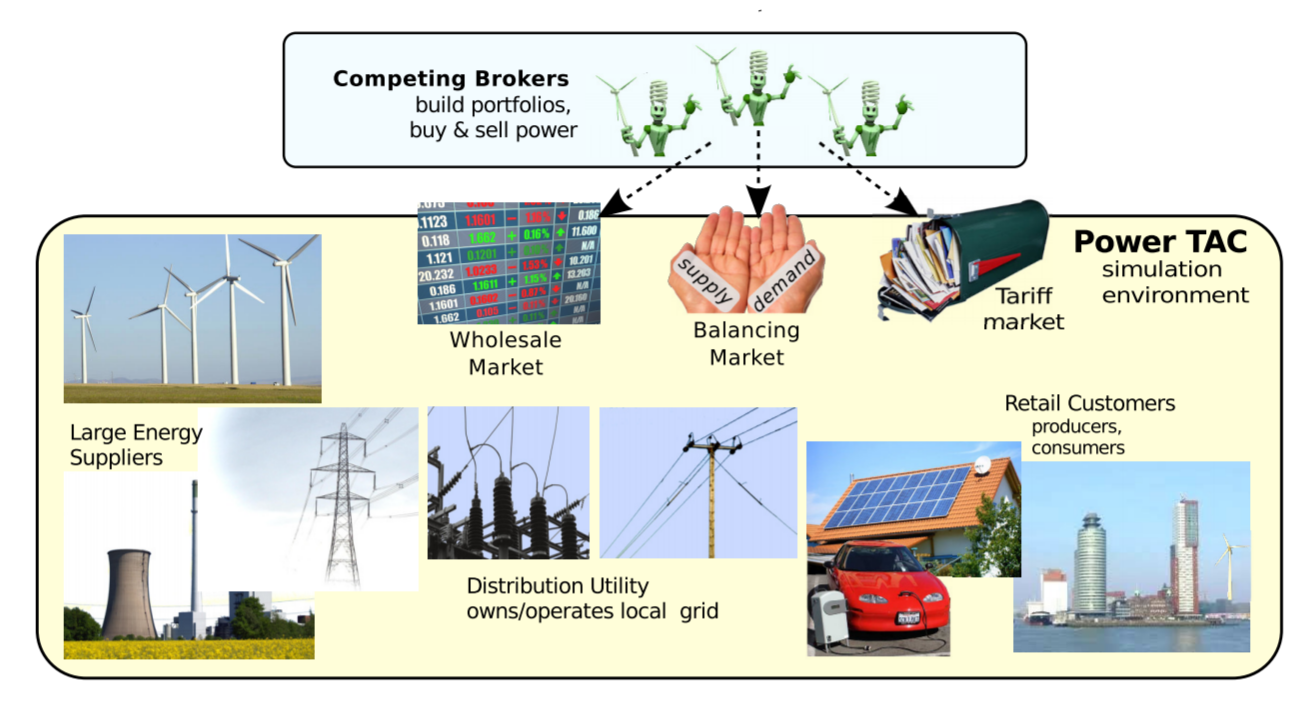
\includegraphics[width=10cm]{img/entorno.png}
	\caption{Elementos del entorno de simulación de Power TAC.}
	\label{entorno}
\end{figure}

A continuación se describen cada uno de los elementos:\\

\textbf{Customer Market.}\\

También conocido como el  Mercado de Tarifas, por este medio los agente adquiere energía eléctrica a través de los productores locales y posteriormente la vende a sus clientes de consumo. El agente adquiere cliente ofreciendo contratos o tarifas en el Mercado de Tarifas especificando el precio de la energía y otros términos, mientras que los clientes tomas la decisión de aceptarlos o ignorar. Los paramentos de una tarifa permite especificar los siguiente términos: periodo de pagos, tiempo de uso, bonos o pagos por suscripción, mínima duración de contrato, pagos de penalización de retiro antes de cumplir con la mínima duración, precio por consumo y producción, etc. Para más información  de la estructura de un tarifa véase la sección \ref{tariff}.

\textbf{Wholesale Market.}\\

Mercado al por Mayor permite a los broker comprar y vender energía entre 1 y 24 horas en el futuro, por este razón también es conocido como Mercado del Día Siguiente. El broker y otros participantes proporcionan energía al por mayor a granel y liquidez al mercado, simulando la demanda de un mercado regional que es sustancialmente mayor que la demanda representada por el escenario de simulación de Power TAC.\\

\textbf{Distribution Utility.}\\

El Distribuidor de Utilidades (DU) modela el monopolio regulador y mantiene la infraestructura de distribución de energía. Dentro del contexto de Power TAC participa en los siguientes escenarios:

\begin{enumerate}
	\item Encargado de distribuir la energía de la red a los clientes. Implicado pagos por el uso de la distribución de la energía hacia los clientes.
	\item Permite importar y exportar energía desde el Mercado al por Mayor.
	\item Actúa como broker de última instancia, ofreciendo sencillas tarifas clientes de consumo y de producción de energía.
	\item Participa en el proceso de balance de la red.
\end{enumerate}

\textbf{Balancing Market.}\\

El mercado de balance es el encargo de mantener el equilibrio entre la oferta y la demanda en la distribución en la red. El Mercado de Balance mantiene un sistema de incentivo para los broker por mantener el equilibrio entre la oferta y la demanda de su portafolio de clientes en cada intervalo de tiempo.\\

\textbf{Accounting.}\\

Para garantizar la coherencia y la imparcialidad, el simulador de Power TAC mantiene un registro de las cuentas de los agentes, las suscripciones de los clientes y las posiciones en el Mercado al por Mayor. Ademas mantiene un registro las siguientes transacciones:

\begin{itemize}
	\item Suscripción y retiro de clientes por tarifa.
	\item Consumo y producción de energía por cliente.
	\item Pagos por publicación de tarifas.
	\item Pagos por distribución.
	\item Pagos del Mercado al por Mayor.
	\item Pagos del Mercado de Balance.    
\end{itemize}

Cada agente tiene una cuenta en efectivo en el banco central, e inicia el juego con un saldo de cero en la cuenta. Los créditos y débitos de las distintas transacciones se agregan a la cuenta durante cada timeslot.\\

\textbf{Weather reports.}\\

El pronostico meteorológico y las condiciones meteorológicas actual se envían a los broker en cada intervalo de tiempo. Algunos modelos de clientes utilizarán esta información para influir en el consumo de energía y en la producción. Los informes meteorológicos y las predicciones se extraerán de los datos meteorológicos y de pronósticos del mundo real para. La ubicación específica y el intervalo de fechas para el conjunto de datos meteorológicos son información privilegiada, no revelada a los agentes, sin embargo se dan la latitud y época del año.\\

\textbf{Tiempo de simulación.}\\

El tiempo de simulación en Power TAC se divide por timeslot cada uno con una duración de una hora en tiempo de simulación, cada timesslot tienen un a duración de 5 segundos en tiempo real, las rondas de simulación consisten en 60 días de simulación equivalente a 1440 timeslot o aproximadamente a 2 horas en tiempo real.\\

\section{Broker.}

El broker es el responsable de ser el intermediario entre las negociaciones en el Mercado de Tarifas, Mercado al por Mayor y el Mercado de Balance, con el objetivo de lograr ganancias a partir de la compra y venta de energía. Durante un times slot el agente puede realizar algunas de las actividades de la figura \ref{activity}.

\begin{figure}[!h]
	\centering
	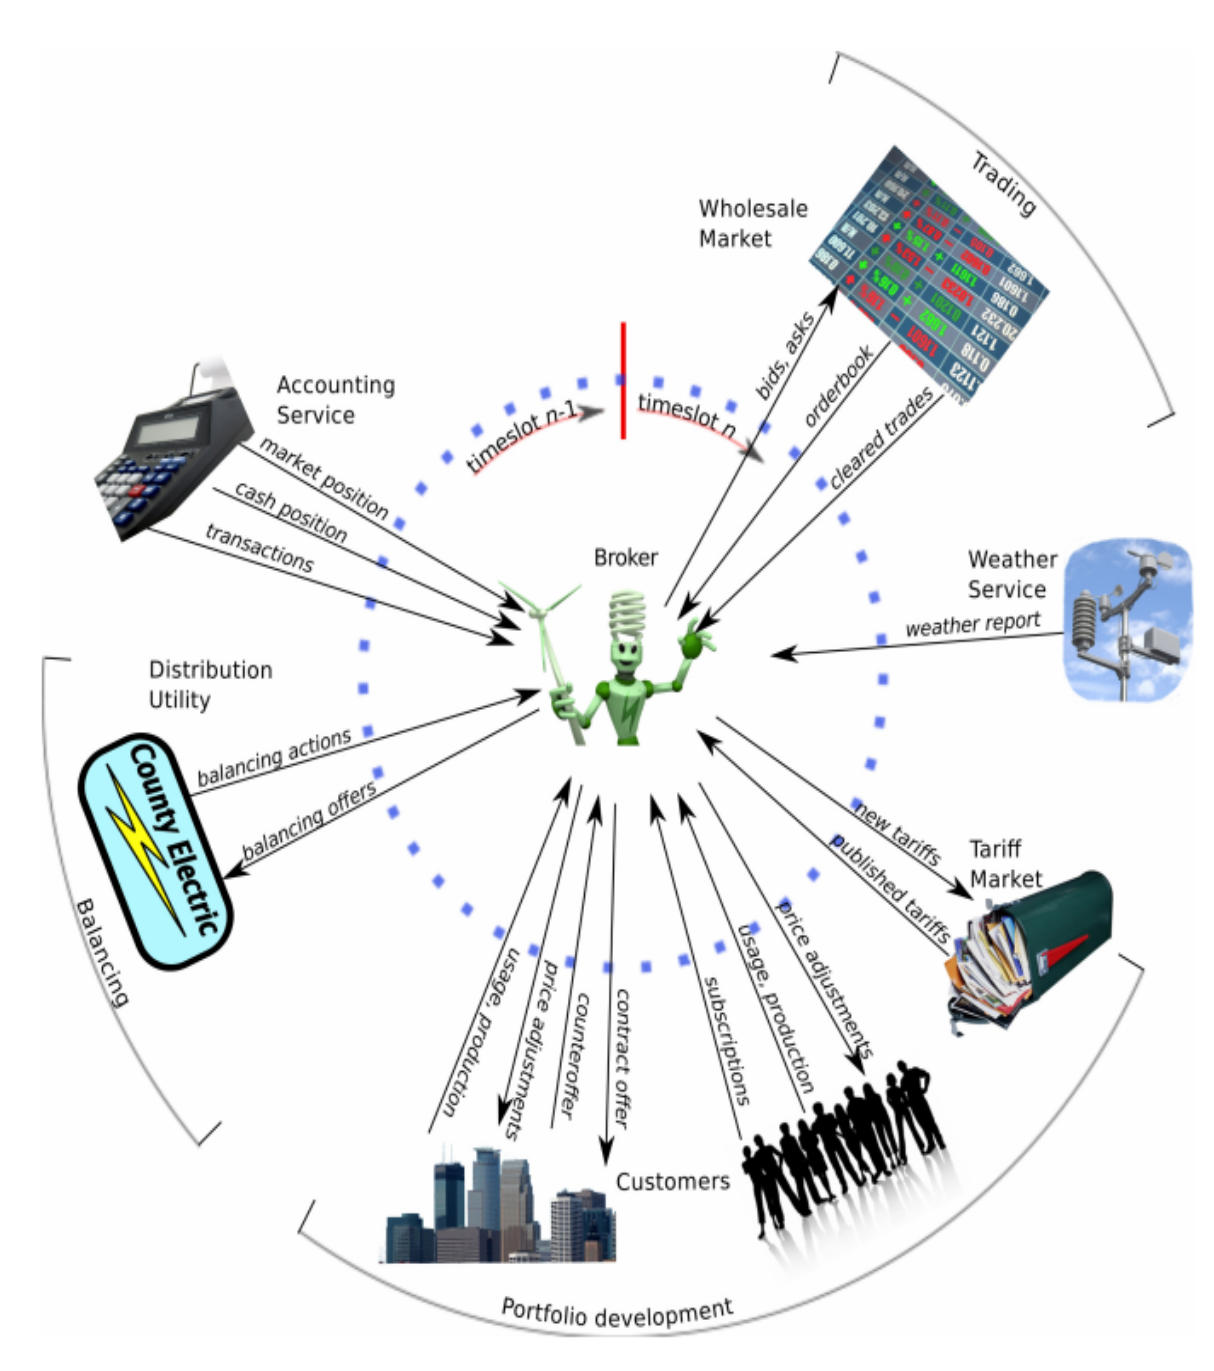
\includegraphics[width=8cm]{img/process.png}
	\caption{Actividades realizadas por el broker en un time slot.}
	\label{activity}
\end{figure}

\begin{description}
	\item [Oferta de tarifas (Mercado de Tarifas):] crea y publica nuevas tarifas.
	\item [Modificación de tarifas (Mercado de Tarifas):]  cambia las condiciones de una tarifa reemplazandola por una nueva.
	\item [Ajuste de precios (Clientes):] ajustar los precios de las tarifas ya existentes.
	\item [Recortar la demanda (Clientes):] para los clientes que han suscrito a las tarifas que permiten capacidades controlables, los broker pueden ejercer restricciones para gestionar la demanda.
	\item [Publicar ordenen de balance (Mercado de Balance):] proporcionar al mercado de balance clientes con capacidades controlables para contribuir al desbalance de la red.
	\item [Enviar solicitudes y ofertas (Mercado al por Mayor):]  crear solicitudes y ofertas para vender y adquirir energía para los futuros timeslot.
\end{description}
\section{Customer.}

Power TAC ofrece modelos de clientes que interactúan con los broker mediante el Mercado de Tarifas. Cada uno de los clientes se caracteriza por un comjunto de información que incluye:

\begin{description}
	\item[Name:] un identificador único.
	\item[Population:] un entero representando el numero de entidades indivisibles (casa, oficinas, vehiculos electricos).
	\item[PowerType:] indica si el cliente es de producion o de consumo, ademas indica si  son controlables o de almacenamiento.
	\item[Controllable capacity:] son indicado por tres atributos: controlableKW  es el total de capacidad en kWh, up-regulation un rango máximo de descarga en kW y down-regulation un rango de máximo en kW de almacenamiento. Si estos tres números están en cero indica que este cliente no tiene capacidades controlables.
	\item[MultiContracting:] es la capacidad del cliente en particionar la población sobre múltiples tarifas.
	\item[CanNegotiate:] este campo indica que el cliente tiene la capacidad de negociar contratos individuales. Este campo por el momento no tiene utilidad para la competencia del 2017.
\end{description}

Cada uno de los clientes representa una población de clientes con características similares, los modelos de clientes realizan tres funciones básicas en el simulador:

\begin{itemize}
	\item Consumen y producen energía.
	\item Evalúan y se suscriben  a tarifas en el mercado de tarifas.
	\item Contribuyen a la demanda de la red, mediante la interrupción o  a la regularización (up-regulation o down-regulation).	
\end{itemize}

\subsection{Storage model.}
Representa un dispositivo de almacenamiento de energía con capacidad para controlar remotamente la carga y/o descarga. Este modelo permite representar el dispositivo de almacenamiento como las baterías, pero también permite representar otros dispositivos de almacenamiento por ejemplo dispositivos de almacenamiento termino. Aunque la diferencia básica entre una batería y un dispositivo de almacenamiento térmico es que el dispositivo de almacenamiento térmico no puede descargarse para obtener energía eléctrica, pero su calor se utiliza para algún propósito (como calefacción, por ejemplo).

\subsection{Capacidades Controlables.}
Capacidades controlables o gestión de la demanda se puede presentar en dispositivos para clientes de producción y de consumo. Los clientes pueden proporcionar a los corredores diferentes formas de capacidades de gestión de la demanda que se pueden utilizar para controlar los costos o para equilibrar, según lo determinado por el PowerType. Estos difieren en la disponibilidad y la cantidad de energía disponible en un intervalo de tiempo. Algunos proporcionan regulación positiva (reducción de la demanda o aumento de la oferta), y algunos proporcionan regulación a la baja. Los dispositivos controlable en general son de dos tipos: 
\begin{enumerate}
	\item Dispositivos que permiten la interrupción del consumo o producción durante un rango asignado.
	\item Dispositivos con características de almacenamiento.
\end{enumerate}

Tres entidades interactúan con el fin de exponer, operar, evaluar y controlar las capacidades controlables: Los clientes, el Broker y el Distribuidor de Utilidades.\\

\textbf{Cliente.}\\

Algunos clinetes ofrecen recursos que pueden ser controlables, y tienen preferencias sobre la conveniencia y precios de energía que afectarán su evaluaciones de las tarifas que proponen ejercer controles.\\

\textbf{Broker.}\\

Los broker pueden estar motivados a crear tarifas para clientes con capacidades controlables o de almacenamiento por las siguientes dos razones:

\begin{enumerate}
	\item Para reducir los costos en el Mercado al por Mayor. Un agente puede ejercer directamente controles para un intervalo de tiempo específico. Estos controles se denominan controles económicos.
	\item Para reducir los cargos por penalización durante el proceso de balance, el broker puede autorizar el DU a ejercer controles sólo en caso de hacerlo sería beneficioso para el corredor. Tales controles se denominan controles de balance.
\end{enumerate}

\textbf{Distribuido de Utilidades.}\\

El DU es el responsable de ejercer efectivamente los dispositivos con capacidades controlables, ya que controla la infraestructura física. Los controles de balance se ejercen después de la ejecución de los modelos de cliente, lo que significa que el DU debe comunicar un mensaje de control a los broker afectados, así como a los clientes. También debe emitir transacciones de tarifas adicionales para cada suscripción de la tarifa afectada.

\section{Tarifas.}
\label{tariff}
Las tarifas son la relación existente entre un broker y sus clientes, es decir es un contrato que especifica una serie de condiciones asociadas al precio, minima duración de contrato, bonos y pagos por suscripción, etc. Los broker son los encargados de crear tarifas específicas a partir de un estructura definida  en la figura \ref{tariff}. La estructura de una tarifa puede variar dependiendo al PowerType que esté sujeta a ella.

\begin{figure}[!h]
	\centering
	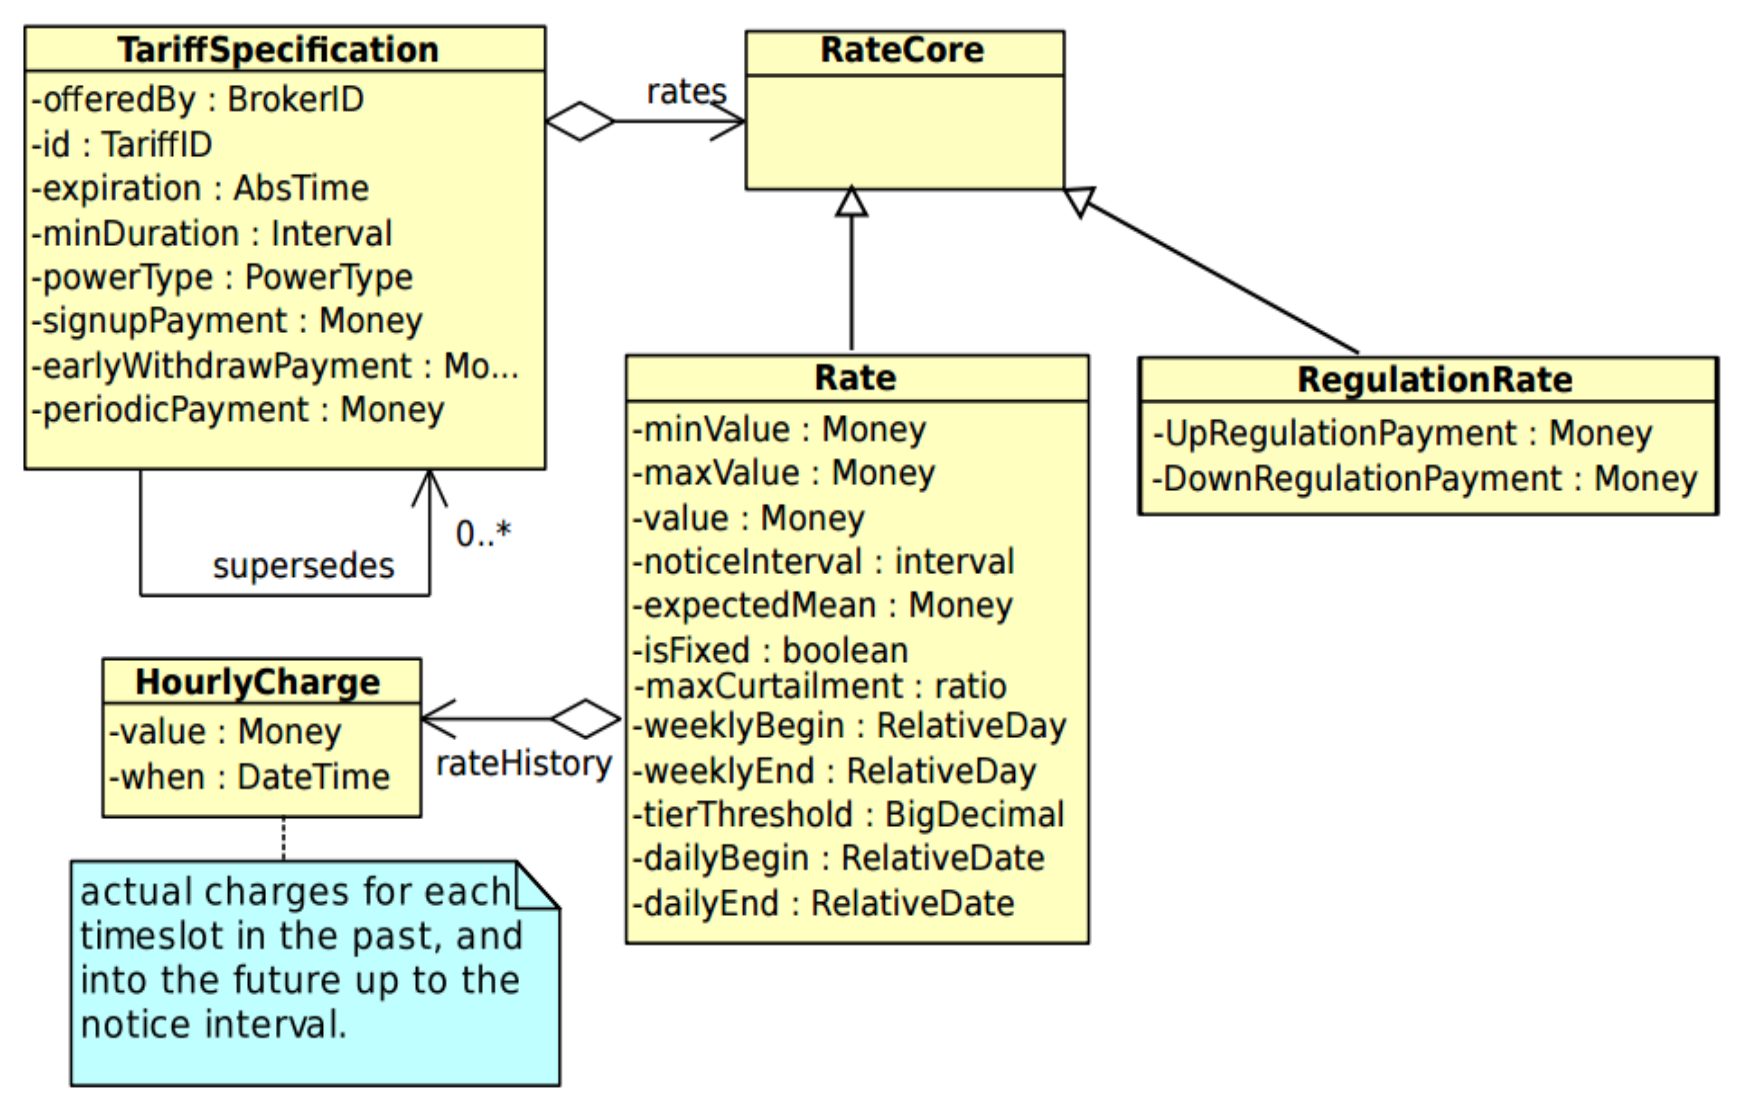
\includegraphics[width=13cm]{img/tariffstructe.png}
	\caption{Clases asociadas a la estructura de una tarifa.}
	\label{tariff}
\end{figure}

Muchos de los elementos de una tarifa son representados por la estructura TariffSpecification donde podemos indicar las condiciones del pago y el PowerType, pero el precio de la energia es definido mediante la estructura Rate. La cantidad de dinero y de energía especificado en TariffSpecification es visto desde el punto de vista de un cliente, es decir  un valor es negativo representa una pago del cliente y el broker, mientras un valor positivo representa un pago desde el broker al cliente. Similar mente una cantidad de energía representado en kWh con un valor positivo representa energía entregada al cliente y un valor negativo es la energía entregada al broker.\\

Cuando el broker publica una tarifa esta debe de pasar por una serie de estados en la figura \ref{state} muestra los estados de un tarifa. El broker envia una tarifa al mercado de tariff y esta entra en estado de “pending”. La nueva tarifas es publica periódicamente a los clientes y a los broker, entrando al estado “Offered”, los clientes se suscribe y la tarifa entra en un estado “active”. Inmediatamente el broker es notificado de varios eventos entre ellos, suscripción de clientes, cancelación de contrato, entre otras acciones. Los tarifas pueden tener una fecha de vencimiento y no se permiten nuevas suscripciones en este caso entra en un estado de “expired” hasta que esta es revocada o modificado por un broker.

\begin{figure}[h!]
	\centering
	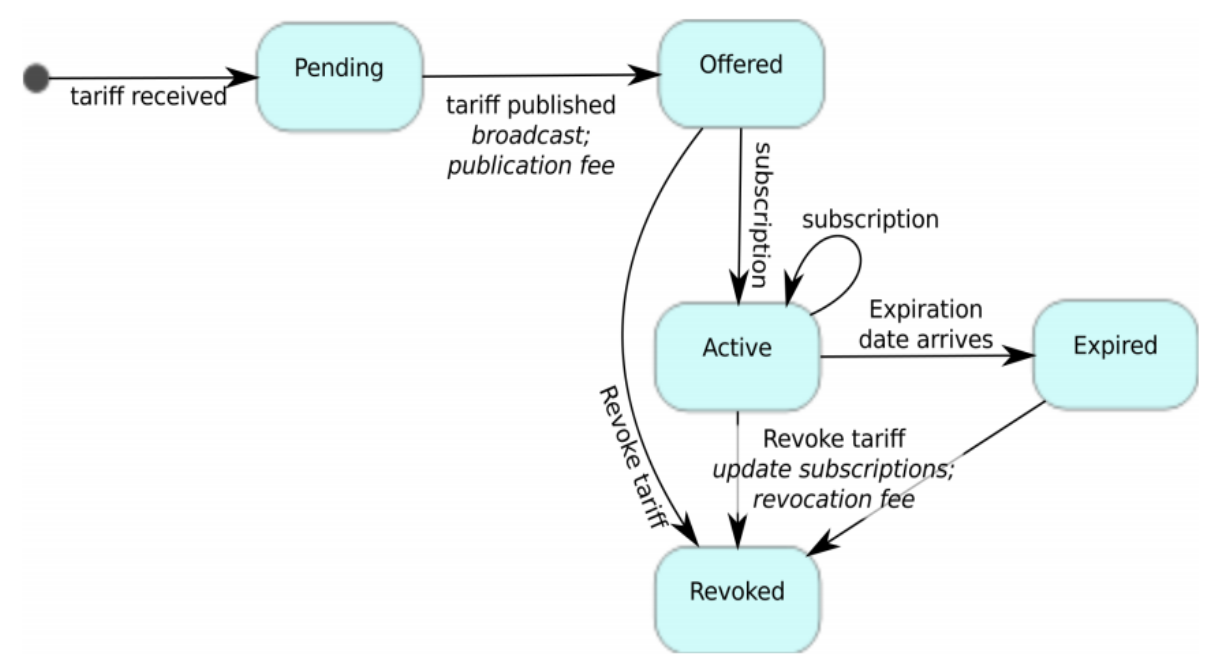
\includegraphics[width=10cm]{img/state.png}
	\caption{Estados de un tarifa.}
	\label{state}
\end{figure}

\subsection{Tarifas para clientes con capacidades controlables.}

Los clientes con capacidades controlables pueden elegir tarifas especificas diseñadas para proporcionar control en los dispositivos o pueden optar por tarifas mas generales que no proporciones un control sobre ellos. La cuestión es como el cliente obtiene beneficios por permitir un control externo. Con los dispositivos de consumo controlable estándar los clientes obtienen un descuento en la tasa de consumo a cambio de permitir la reducción del consumo. Pero este esquema no parece adecuado para clientes con dispositivos de almacenamiento, una solución es pagar o cobrar al clientes por las acciones de carga y descarga de sus dispositivos. En la construcción de una tarifa para clientes con capacidades controlables se puede incluir términos de interrupción y de regularización a partir de una estructura externa a TariffSpecification, empleando la estructura Rate y RegulationRates definimos los términos antes mencionados. Los clientes interrumpibles permiten que una porción de consumo o producción del cliente se reduzca durante una porción del intervalo de tiempo para reducir los costos generales de energía y para reducir costos del desbalance. La estructura de de RegulationRates permite incluir un valor para especificar un tasa de interrupción durante un timeslot, agregando un valor distinto de cero en la propiedad de maxCurtaiment dentro de la estructura del Rate. Para los cliente con capacidades de almacenamiento, dentro de la estructura RegulationRates se puede incluir términos para los pagos por el uso del dispositivo durante un desbalance negativo (up-regulation) o un desbalance positivo (down-regulation).

\section{Información disponible para los broker.}

El servidor de Power TAC durante un juego proporciona información del entorno de simulación a los broker, esta informacion es enviado a partir de mensaje  asincronos y puede ser pública o privada.\\

Al inicio de la simulación el broker recibe la siguiente información:
\begin{description}
	\item [Game parameters: ]parámetros usados para la configuración o instancia de un específico juego.    
	\item [Broker Identities: ]username de los broker participantes en el juego.
	\item [Customer Records: ]nombres y características de los modelos de clientes ejecutando durante la simulación.
	\item [Default tariff: ]al iniciar el juego, el mercado de tarifas solo oferta tarifas publicadas por el default broker.
	\item [Bootstrap Customer Data: ]consumo y producción de cada uno de los clientes durante un periodo de 14 días antes de iniciar la simulación.
	\item [Bootstrap Market Data: ]precios y cantidades de energía comprada por el Default Broker en el Mercado al por Mayor durante los 14 días anteriores al inicio de la simulación.
	\item [Bootstrap Weather data: ]reportes del clima durante los 14 días antes del inicio de la simulación.
	\item [Weather report, Weather forecast: ]predicciones del clima en las siguientes 24 horas.  
\end{description}
La siguiente información se envía a los corredores una vez cada 6 horas de simulación, cuando se publican las tarifas:
\begin{description}
	\item [Tariff updates: ]las siguiente acciones creación de nueva tarifa, revocar una tarifa y sustituir una tarifa, se les notificará a cada uno de lo broker.
	\item [Tariff transactions:] Cuando se publica una tarifa de un broker, se  cobra un bono por publicación, cuando los clientes  cambian la suscripción, los broker reciben transacciones que describen los cambios junto con una bonificación y la cantidad de penalizaciones de salida anticipada. Esta informacion es privada y solo para el propietario de la tarifa.
\end{description}
La siguiente información es publica y se enviá a cada uno de los broker en cada time slot.
\begin{description}
	\item [Wholesale market clearing data: ]los precios de compensación del mercado y las cantidades totales negociadas para cada una de las 24 oportunidades de negociación en el Mercado al por Mayor. Estos mensajes pueden omitirse si no se hicieron operaciones en un intervalo de tiempo dado.
	\item [Wholesale market orderbooks: ]contiene precios y cantidades de todas las ofertas y solicitudes no satisfechas.
	\item [Total aggregate energy consumption: ]producción y consumo total de energía para el intervalo de tiempo actual.
	\item [Wheather report and weather forecast:] condiciones meteorológicas para el intervalo de tiempo actual y pronóstico para las próximas 24 horas.
\end{description}
Cada vez que se ejecuta la evaluación de demanda máxima una vez por semana, cada broker recibirá un conjunto de mensajes de Capacity transactions, una para cada pico de demanda evaluado. Estas transacciones especifican el umbral de demanda, la contribución del broker al pico de energía y la cuota asociada. La siguiente información es privada y enviado individualmente a cada broker en cada time slot.
\begin{description}
	\item [Tariff transactions:] Lecturas de créditos y débitos asociados a los clientes.
	\item [Balancing and distribution transactions:] Cargos por el DU para cada broker individual para compensar el Mercado de Balance y la distribución de energía.
	\item [Portafolio supply and demand:] Transacciones de producción y consumo de los clientes actuales del broker.
	\item [Wholesale market transations:] ofertas y presentadas por el broker.
	\item [Market Positions:] los compromisos netos actualizados de importación / exportación del Broker, para cada una de las 24 oportunidades de negocio en el Mercado al por Mayor.
	\item [Cash Position: ]actualización de la cuenta bancaria del Broker después de que todas las transacciones contables vigentes se han aplicado.
\end{description}

\section{Wholesale Market.}

\section{Balance Market.}

El Mercado de Balance debe satisfacer tres objetivos:
\begin{enumerate}
	\item El consumo total de energía neta debe sumar a cero una vez que el mercado se ha liquidado.     
	\item Cada broker que tiene un tiene un balance positivo debe tener recursos de producción controlables reducidos, o debe ser pagado por su exceso de energía por una tasa determinada por el proceso de balance del mercado.      
	\item Cada broker que tiene un balance negativo debe tener recursos controlables de consumo reducido, o debe pagar por la energía adicional necesaria.	
\end{enumerate}

\section{Distribuidor de Utilidades.}
El DU opera la red de distribución que conecta la red de transmisión al por mayor de los agentes y clientes. También actúa como el “agente por defecto", ofreciendo tarifas básicas y poco atractivas para todos los tipos de clientes. Los  costos del DU deben ser cubiertos por los honorarios pagados por los agentes a través de las comisiones de distribución y de regularización. Con capacidad controlable, los broker pueden presentar órdenes de balance que le permiten al DU ejercer control de capacidad para lograr el equilibrio. Los broker deben presentar sus órdenes de balance antes de que se ejecuten los modelos de cliente y el DU ejecuta su proceso de balance después de que se conozca el consumo del cliente para el intervalo de tiempo actual. El DU puede determinar las cantidades reales disponibles para cada orden de balance.

\section{Procesos de Decisión de Markov.}
Las técnicas Markovianas modelan un problema de decisión secuencial, definido por un conjunto de estados, un conjunto de acciones posibles, un modelo del entorno y una función de recompensas, que sirve como medio de interacción entre el entorno y el agente. Sus dominios se modelan como sistemas estocásticos, sus metas se definen por sus funciones utilidad/coste (recompensa/descuento), donde el problema de planificación se transforma en un problema de optimización. De ahí que su solución sea la política óptima, asignando la mejor acción en cada estado del espacio de estados del problema.\\

Al problema de encontrar una estrategia reactiva de control (o política de acción) en problemas de decisión secuencial, que maximice la recompensa esperada en el tiempo, se le conoce como proceso de decisión de Markov o MDP (por sus siglas en inglés Markov Decision Process). El trabajo de Markov supone que el agente siempre conoce el estado en que se encuentra al momento de iniciar la ejecución de sus acciones y que la probabilidad de transición depende solamente de este estado y no de su historia, es decir cumple con la propiedad de Markov\footnote{La Propiedad de Markov se refiere a la propiedad de ciertos ambientes estocásticos, donde la distribución de la probabilidad del valor futuro de una variable aleatoria depende únicamente de su valor presente, siendo independiente de la historia de dicha variable.}, afectada por un factor de descuento que impacta negativamente a la utilidad

\subsection{Definición Matemática.}
Los MDPs proveen un marco matemático intuitivo para modelar problemas de decisión secuencial en ambientes dinámicos inciertos . Formalmente un MDP es una 4-tupla:
$$M=< S,A,T,R >$$
Donde:\\
$S$ = conjunto de estados $\{s_{1},...,s_{n}\}$.\\
$A$ = conjunto de acciones $\{a_{1},...,a_{n}\}$.\\
$T$ = función de transición de un estado $s$ a $s'$.\\
$R$ = función de recompensa de un estado $s$ a $s'$ mediante una acción.\\

\section{Métodos de Resolución.}
Recordemos que la tarea del agente es encontrar una política que maximice alguna medida de refuerzo. Su optimización conduce a la obtención de un sistema de ecuaciones no lineales debido a que contienen una maximización. Existen varios métodos de resolución de MDPs, basándose en el conocimiento completo del MDP se clasifican de la siguiente forma:

\begin{itemize}
	\item Programación dinámica.
	\item Programación lineal.
	\item Aprendizaje por refuerzo.
\end{itemize}

La primeras dos técnicas se distingue por conocen el MDPs, es decir tienen conocimiento del conjunto de estado, conjunto de acciones, de la función de transición y la función de recomienza. En cambio la tercera no tiene acceso a esta información, por lo que requiere explorar para aprender estados probables, resultando por ello más compleja que las dos primeras y con la posibilidad de que no se cumpla con la propiedad de Markov.

\subsection{Programación Dinámica.}
La programación dinámica se basa en el principio de optimalidad de Bellman\footnote{Principio de Optimalidad de Bellman: "dada una secuencia óptima de decisiones, toda subsecuencia de ella es, a su vez, óptima"}, lo que tratan de conseguir los algoritmos de programación dinámica es el mantenimiento de las funciones de valor $V (s)$ o $Q(s, a)$ de forma que una vez obtenidos los valores óptimos de estas funciones se pueda derivar de ellas la política óptimas.\\

Los distintos enfoques de programación dinámica explícitamente almacenan funciones de valor del espacio de estados e iterativamente actualizan los valores para cada estado, hasta que el cambio de la función de valor es menor o igual al umbral previamente establecido. Entonces se dice que la función de valor converge a su valor óptimo, con su correspondiente acción o política óptima. Por lo que la programación dinámica ofrece un enfoque unificado para resolver problemas de control estocástico como lo son los MDPs. Los métodos más populares de programación dinámica son el algoritmo de iteración de valor y el algoritmo de iteración de política.

\subsubsection{Iteración por Valor.}
El algoritmo de iteración de valor aplica actualizaciones sucesivas de la función de valor para cada estado $s \in S$, al ejecutar el Principio de Optimalidad de Bellman, siendo la recompensa inmediata del estado en evaluación su valor inicial. De esta manera se actualiza la utilidad de cada estado a partir de las utilidades de sus estados vecinos inmediatos. Entonces se repite el proceso hasta que alcanza la convergencia. Cabe destacar que si esta actualización se aplica indefinidamente, entonces queda garantizado que se alcanzará un estado de equilibrio. El proceso se detiene cuando la diferencia entre las dos últimas iteraciones es menor que el máximo error permitido. Entonces, la iteración de valor converge finalmente a un único conjunto de soluciones. A continuación se muestra el algoritmo de Iteración por Valor.

\subsubsection{Iteración por Política.}

Una política $\pi$ define el comportamiento de un agente aprendiz en un momento dado. En otras palabras, una política es un mapeo de un conjunto de estados $S$ percibidos del ambiente a un conjunto de acciones $A$ que deben ejecutarse en dichos estados. En algunos casos la política puede ser una función simple o una tabla de entradas, y en otros casos puede ser un proceso complejo de búsqueda. En general, las políticas pueden ser estocásticas.

$$\pi : S \rightarrow A$$\\

Otro algoritmo de programación dinámica es la iteración de política, en este método, la política es repetidamente mejorada al encontrar una acción en cada estado que tenga un valor más alto que el valor de la acción escogida anteriormente para ese estado. La política inicial es aleatoria y el proceso termina cuando ya no es posible realizar más mejoras. Cabe señalar que este proceso garantiza la convergencia a la política óptima.
La dinámica de este algoritmo es la siguiente: toma al MDP, a un valor de descuento, a un parámetro de convergencia y produce políticas óptimas de horizonte finito sucesivas, terminando cuando el máximo cambio entre la función del valor actual y la del valor previo es menor que el margen de error dado. De esta manera logra la convergencia y se detiene. A continuación se muestra el algoritmo de Iteración por Políticas:

\subsection{Programación Lineal.}

Esta técnica resuelve un problema indeterminado formulado a través de ecuaciones lineales, para ello cuenta con el método Simplex. Este método fue desarrollado por G. B. Dantzig en 1947 y consiste en la optimización de la función objetivo al considerar las restricciones habidas. Estas restricciones son desigualdades que acotan a la región que contiene a todos los valores factibles para dichas expresiones matemáticas. Con este método, la iteración toma el valor de un vértice e investiga si es su máximo valor, de no ser así repite el proceso en forma iterativa hasta encontrarlo.

\section{Aprendizaje por Refuerzo.}
El aprendizaje por refuerzo consiste en aprender qué acciones realizar, dado el estado actual del ambiente, con el objetivo de maximizar una se\~{n}al de recompensa numérica, lo cual requiere de un mapeo de situaciones a acciones. El sistema que aprende debe descubrir por sí solo cuales son las acciones que le dan a ganar más. En los casos más interesantes y difíciles, las acciones pueden afectar no sólo la recompensa inmediata sino también la siguiente situación,y de esta forma afectar las siguientes recompensas. Estas dos características, prueba y error, y recompensas retrasadas, son las dos características más sobre salientes del aprendizaje por refuerzo.\\

En caso de que no se cuente con la función de transición de estados ni con la función recompensa del problema, el planificador deberá explorar su entorno para aprender qué hacer y cómo relacionar situaciones (estados) con acciones, de manera que la recompensa sea maximizada. El aprendizaje por refuerzo está basado en la interacción constante de un agente con su entorno incierto, por lo que existe un fuerte compromiso exploración-explotación: la información de entrada es la retroalimentación que obtiene del mundo exterior como respuesta a sus acciones. De ahí este aprendizaje sea cercano a la teoría óptima de control y la aproximación estadística.\\

Mediante la función de aprendizaje por refuerzo, el agente determina cuáles estados son más provechosos a corto plazo. A diferencia de la técnica anterior, la función evaluación es hecha a largo plazo, considerando a los estados a los que puede conducir una acción. De esta manera, sus programas de cómputo buscan ir aprendiendo por sí solos conforme van adquiriendo experiencia, tal y como sucede con el ser humano. En consecuencia, los métodos de solución que utilizan aprendizaje por refuerzo son inductivos. La idea central es hacer uso de la estructura inherente de los MDPs, cuyos estados y acciones pueden ser abstraídos en subpolíticas. Una vez que explora y obtiene información de su entorno, este método se torna informado, pudiendo ser resuelto mediante los métodos de programación dinámica o programación lineal antes descritos.\\

A continuación se muestran los algoritmos que se emplean para aprender la dinámica del entorno:
\begin{itemize}
	\item Algoritmos de Equivalencia de Certeza.
	\item Dyna-Q.
	\item Queue-Dyna.
	\item Métodos de Monte Carlo.
	\item Métodos de diferencia temporal.
\end{itemize}

Desde el punto de vista del uso que se haga de la política que se está aprendiendo los métodos de este enfoque se pueden clasificar adicionalmente en:
\begin{itemize}
	\item Métodos on-policy.
	\item Métodos off-policy.
\end{itemize}
%\begin{table}[h!]
% \begin{center}
% \begin{tabular}{|l|l|l|l|l|} \hline
% Minimun\\
% Duration
% &
% PowerType
% &
% Signup Paymen
% &
% Early Withdraw Payment
% &
% Periodic Payment\\
% \hline
% \end{tabular}
% \caption {Clasificación de acuerdo al numero de atributos.}
% \label{clasA}
% \end{center}
% \end{table}